\documentclass[12pt]{article}

\usepackage{sbc-template}
\usepackage{graphicx,url}
\usepackage[utf8]{inputenc}
\usepackage{fancyhdr}
\usepackage[brazil]{babel}
\usepackage{hyperref}
\usepackage{xcolor}
\usepackage{nameref}
%\usepackage[latin1]{inputenc}  

\pagenumbering{gobble}                          % sets page numbering off
\pagestyle{fancy}\setlength\headheight{100pt}   % set the pagestyle to fancy to include headers and footers
\pagestyle{fancy}\setlength\textheight{650pt}
\pagestyle{fancy}\setlength\footskip{20pt}
\fancyhf{}                                      % clear the header and footer
\renewcommand{\headrulewidth}{0pt}              % no horizontale ruler under header
\fancyhead[L]{
\includegraphics[width=3.8cm]{img/LogoINCT.jpg}}
\fancyhead[R]{
\includegraphics[width=3.8cm]{img/LogoOdissea.jpg}}

\begin{document} 

%\title{Guia para o carregamento de dados no Geonode Odisseia}
%\date{}
%\maketitle
%\thispagestyle{fancy}

\begin{center}
  \vspace{12pt}
  \Large\textbf{Guia para construção de Geostories no Geonode}
\end{center}

\section{Introdução}

  Este documento explicita as funcionalidades dos Geostories do Geonode e traz
  instruções para o seu uso. As informações aqui contidas são provenientes das
  documentações oficiais do 
  \textcolor{blue}
  {\href{https://docs.geonode.org/en/master/usage/geostory/index.html}
  {Geonode}}
  e do 
  \textcolor{blue}
  {\href{https://docs.mapstore.geosolutionsgroup.com/en/latest/user-guide/exploring-stories/}
  {MapStore}}.

\section{Criação} \label{sec:firstpage}

  Para criar um novo Geostory siga até a aba "Dados/Conjuntos de Dados" ou
  "Geostories" no menu superior esquerdo (Figura \ref{fig:criar}.1). No
  catálogo de dados ou de geostories clique em "Adicionar Recurso/Criar
  Geostory" (Figura \ref{fig:criar}.2).

  \begin{figure}[ht]
    \centering
    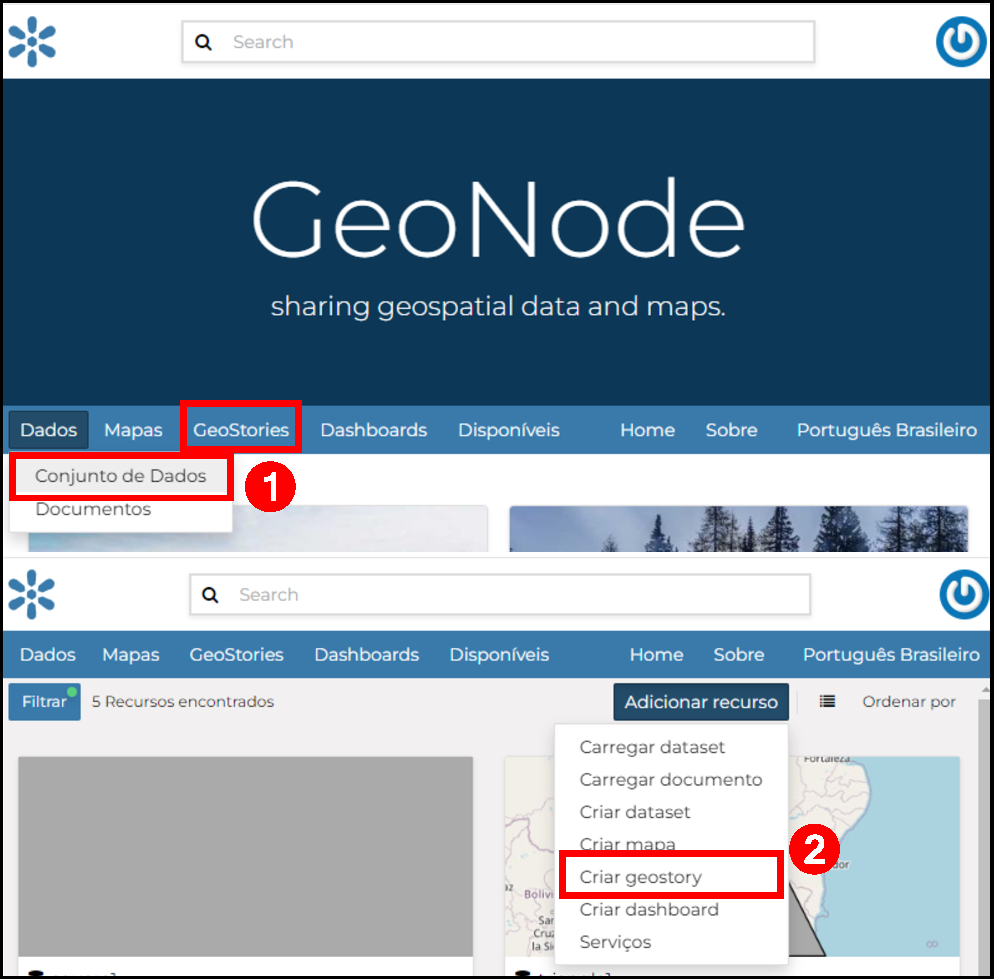
\includegraphics[width=\textwidth, keepaspectratio]{img/criarGeostory.pdf}
    \caption{Fluxo para a criação de um novo Geostory.}
    \label{fig:criar}
  \end{figure}

  Uma vez na tela de criação de Geostory é possível visualizar, na aba
  esquerda, o construtor onde o usuário pode organizar os elementos do Geostory
  e, na aba direita, o contêiner de seções utilizado para criar e editar os
  elementos do Geostory (Figura \ref{fig:overview}). Para criar uma seção
  utilize o botão de "+" na parte inferior do contêiner de seções e selecione a
  seção que deseja criar (Figura \ref{fig:overview}).

  \begin{figure}[ht]
    \centering
    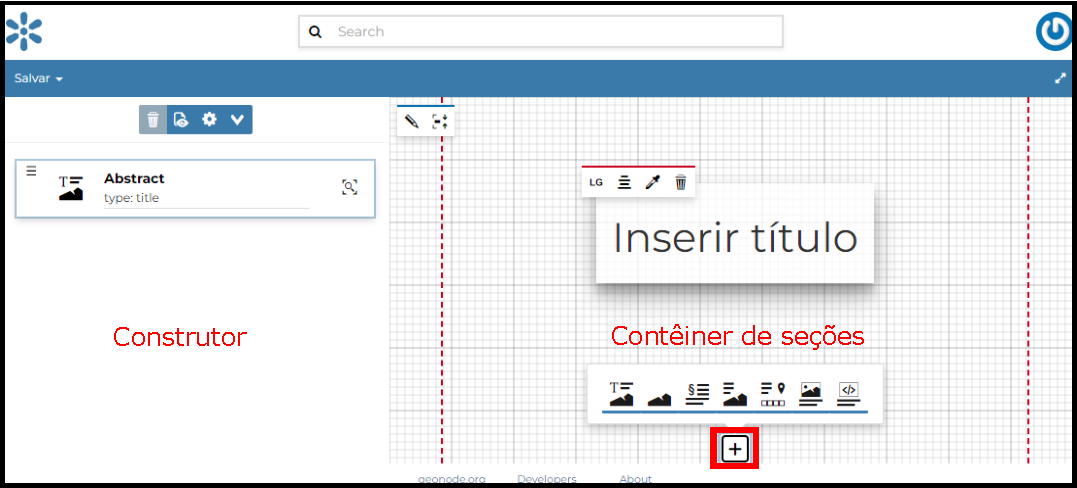
\includegraphics[width=\textwidth, keepaspectratio]{img/overviewGeostory.pdf}
    \caption{Interface gráfica de criação do Geostory em destaque o botão de mais que adiciona seções à página.}
    \label{fig:overview}
  \end{figure}

\section{Tipos de Seção}

\subsection{Título}
  Ao criar um Geostory uma seção de título é adicionada por padrão. Esta
  seção é composta por dois elementos: o título e o plano de fundo. O título é
  uma caixa de texto onde é possível inserir texto e modificar posição,
  tamanho, fonte, cor e outros atributos. Já o plano de fundo é formado por um
  objeto multimídia que irá ocupar o restante do campo de visão da seção.

  Para editar o campo de texto basta clicar sobre a caixa de texto e digitar o
  título desejado. A mudança de atributos do texto devem ser realizadas através
  dos botões da parte superior da caixa de texto (Figura \ref{fig:titulo}).

  Para editar o plano de fundo da seção, o menu de mídia deve ser acessado
  através do botão de edição no canto superior esquerdo do contêiner de seção.
  Este menu possui uma funcionalidade semelhante à seção de multimídia. Também
  é possível retrair a extensão desta seção para a extensão do seu conteúdo
  utilizando o botão no canto superior esquerdo do contêiner de seção (Figura
  \ref{fig:titulo}).

  \begin{figure}[ht]
    \centering
    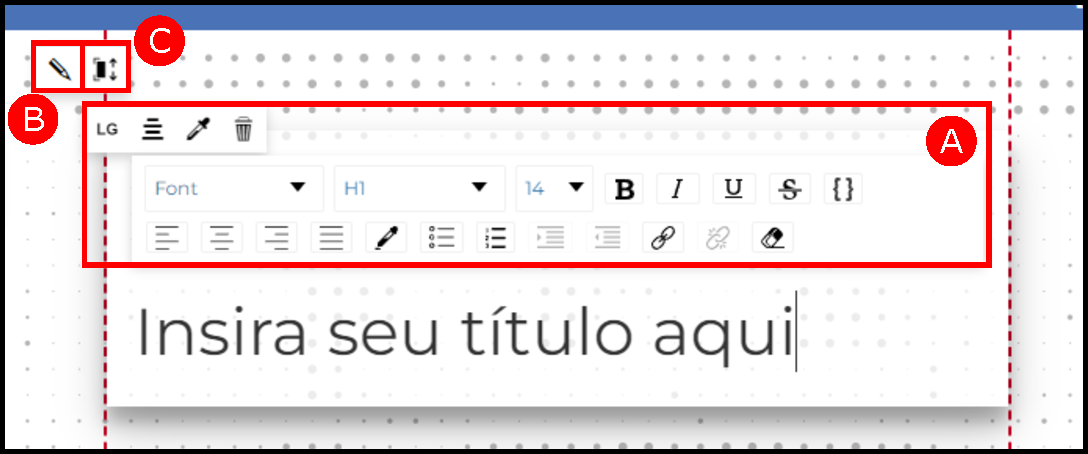
\includegraphics[width=\textwidth, keepaspectratio]{img/tituloGeostory.pdf}
    \caption{Interface de edição da seção de título do Geostory.}
    \label{fig:titulo}
  \end{figure}

\subsection{Multimídia}
  A seção de multimídia é capaz de adicionar imagens, vídeos e mapas presentes
  no Geonode como uma seção em seu Geostory. Também é possível adicionar uma
  imagem ou um vídeo através de sua URL. Para adicionar um elemento presente no
  Geonode, basta selecionar o Geonode como a fonte de recursos no canto
  superior direito do menu multimídia, procurar por seu título na aba de
  filtro, clicar sobre o elemento e adicionar (Figura \ref{fig:midiageonode}).
  No caso de elementos externos, o usuário deve selecionar "Recursos do Story"
  como fonte, acionar o botão de "+", inserir a URL no campo "Fonte" e salvar o
  novo elemento (Figura \ref{fig:midiaexterna}).

  \begin{figure}[ht]
    \centering
    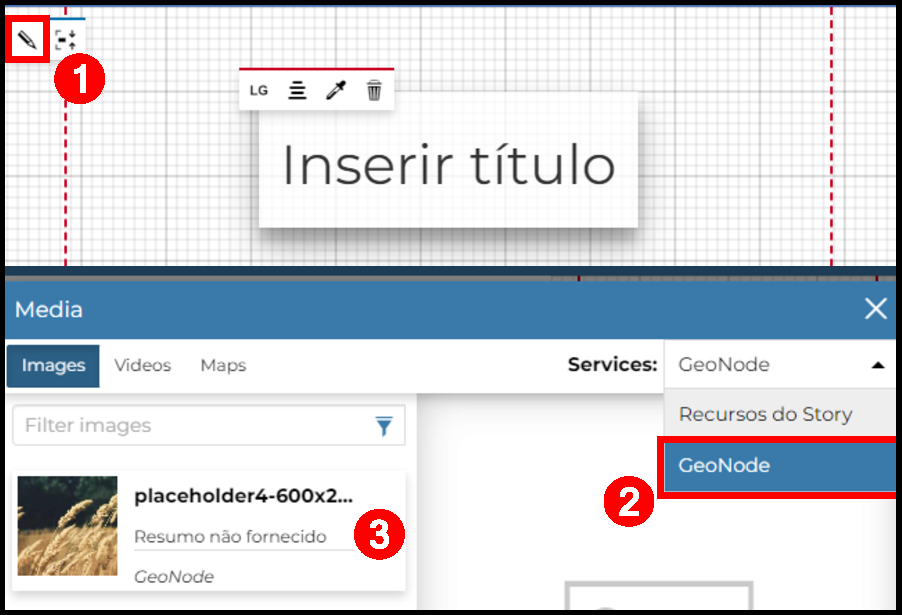
\includegraphics[width=\textwidth, keepaspectratio]{img/midiaGeonode.pdf}
    \caption{Interface gráfica de inserção de mídias do Geonode.}
    \label{fig:midiageonode}
  \end{figure}

  \begin{figure}[ht]
    \centering
    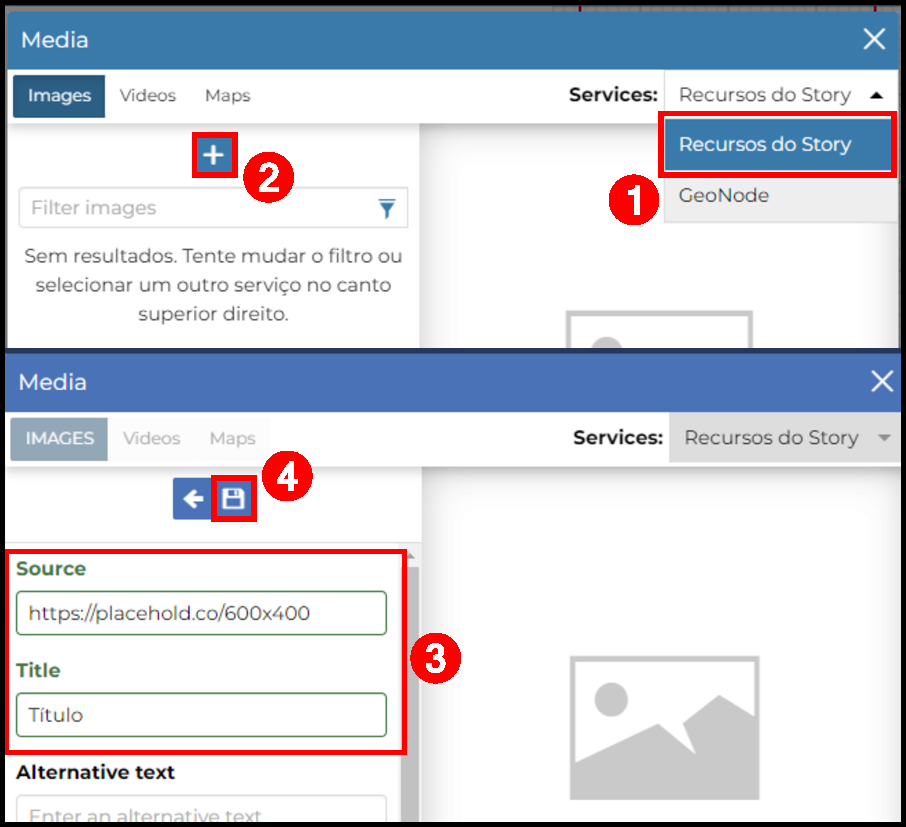
\includegraphics[width=\textwidth, keepaspectratio]{img/midiaExterno.pdf}
    \caption{Interface gráfica de inserção de mídias externas.}
    \label{fig:midiaexterna}
  \end{figure}

\subsection{Web}
  Esta seção permite a visualização de uma página da internet dentro do seu
  Geostory. A página estará contida dentro de um intervalo do Geostory e será
  possível interagir com ela normalmente. Para adicionar uma página basta
  adicionar uma seção de web e inserir a URL da página.

\subsection{Banner}
  A seção de Banner se assemelha com uma seção de título com exceção da
  ausência de uma caixa de texto. Esta seção, portanto, tem como objetivo
  adicionar elementos multimídia entre suas seções.
  
  Para adicionar ou alterar o elemento de multimídia do banner deve-se usar o
  botão de editar no canto superior direito do contêiner de seção e seguir um
  fluxo semelhante à seção de multimídia. Através do botão de
  ajuste de altura é possível modificar a extensão deste contêiner.

\subsection{Parágrafo}
  A seção de Parágrafo permite ao usuário adicionar conteúdo de texto e inserir
  elementos de multimídia e páginas web de maneira integrada. 

  A seção de parágrafo funciona como um sub-contêiner, sendo possível inserir
  texto e multimídia dentro de um parágrafo. As seções podem ser adicionadas
  usando o botão "+" dentro do contêiner. Imagens, mapas, vídeos e páginas web
  serão adicionadas continuamente com o texto.

\subsection{Imersão}
  A seção imersiva permite a apresentação do conteúdo de um parágrafo sobre um
  elemento multimídia. O usuário pode modificar o elemento multimídia de plano
  de fundo utilizando o botão de editar no canto superior esquerdo do contêiner
  de seções e é possível adicionar mais elementos de parágrafo utilizando o
  botão "+" na caixa de texto.

\subsection{Geocarousel}
  A seção Geocarousel cria uma interface do tipo carrossel onde o usuário pode
  navegar por pontos pré-determinados de um dado espacial e adicionar conteúdo
  textual e multimídia em cada um deles.

  Esta seção é composta por três elementos: o mapa de fundo, o conteúdo
  descritivo e o carrossel. O mapa de fundo pode ser modificado através do
  botão de editar no canto superior esquerdo do contêiner de seções. O conteúdo
  descritivo se comporta como uma seção de parágrafo. Já o carrossel é definido
  por um título e uma Thumbnail que deve ser inserido como um arquivo de imagem
  (.jpeg, .png e outros) no momento de sua criação.

  \textbf{Atenção, só será possível adicionar um novo cartão após adicionar um
  marcador no mapa para o cartão atual (Figura \ref{fig:geocarousel}).}

  \begin{figure}[ht]
    \centering
    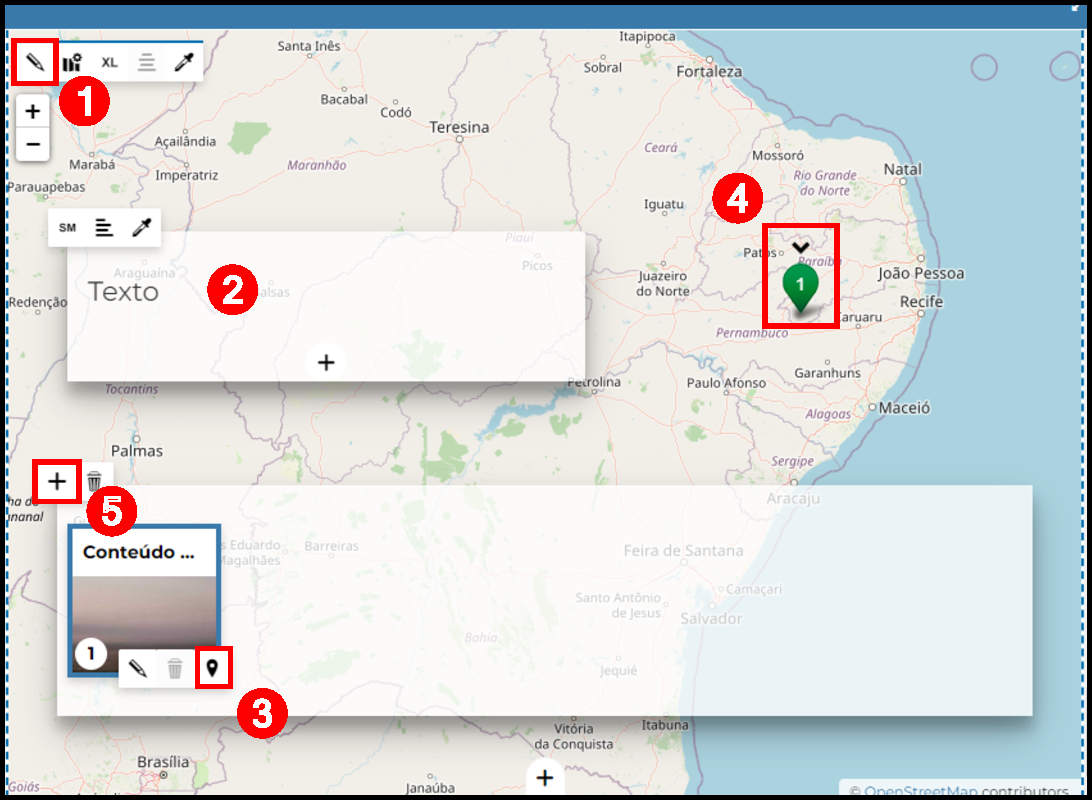
\includegraphics[width=\textwidth, keepaspectratio]{img/geocarrousselGeostory.pdf}
    \caption{Fluxo de criação de um Geocarousel.}
    \label{fig:geocarousel}
  \end{figure}


\section{Organização}
  O construtor permite que o usuário reorganize a ordem das seções do Geostory
  bem como navegue por ele. Utilizando o botão de arrastar no canto superior
  esquerdo de cada seção é possível modificar a ordem dos elementos criados
  anteriormente e utilizando o ícone da lupa no canto direito de cada seção é
  possível mover a visualização até aquele elemento.

  Na parte superior do construtor o usuário pode apagar uma seção selecionada
  através do ícone da lixeira. Uma prévia do Geostory pode ser acessada através
  do ícone de previsão, para retornar ao editor utilize o ícone de edição no
  canto superior esquerdo da página (Figura \ref{fig:previa}).

  \begin{figure}[ht]
    \centering
    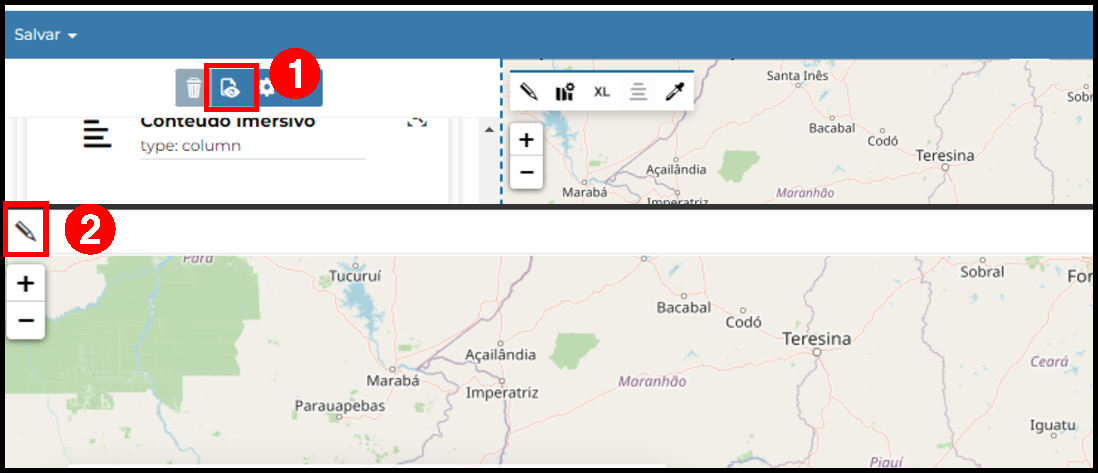
\includegraphics[width=\textwidth, keepaspectratio]{img/visualizacaoGeostory.pdf}
    \caption{Entrada e saída do modo de prévia.}
    \label{fig:previa}
  \end{figure}

\section{Configuração}
  Na parte superior do construtor através do ícone de engrenagem é possível
  acessar o menu de configuração. Este permite que o usuário modifique a
  temática geral do Geostory, como cores do plano de fundo, fonte e cores do
  texto e sombreamento das caixas de texto. O usuário também pode adicionar
  elementos na interface gráfica como título da página, logo e atalhos de
  navegação. Cada seção selecionada nas configurações irá criar um atalho de
  navegação no topo da página (Figura \ref{fig:navegacao}).

  \begin{figure}[ht]
    \centering
    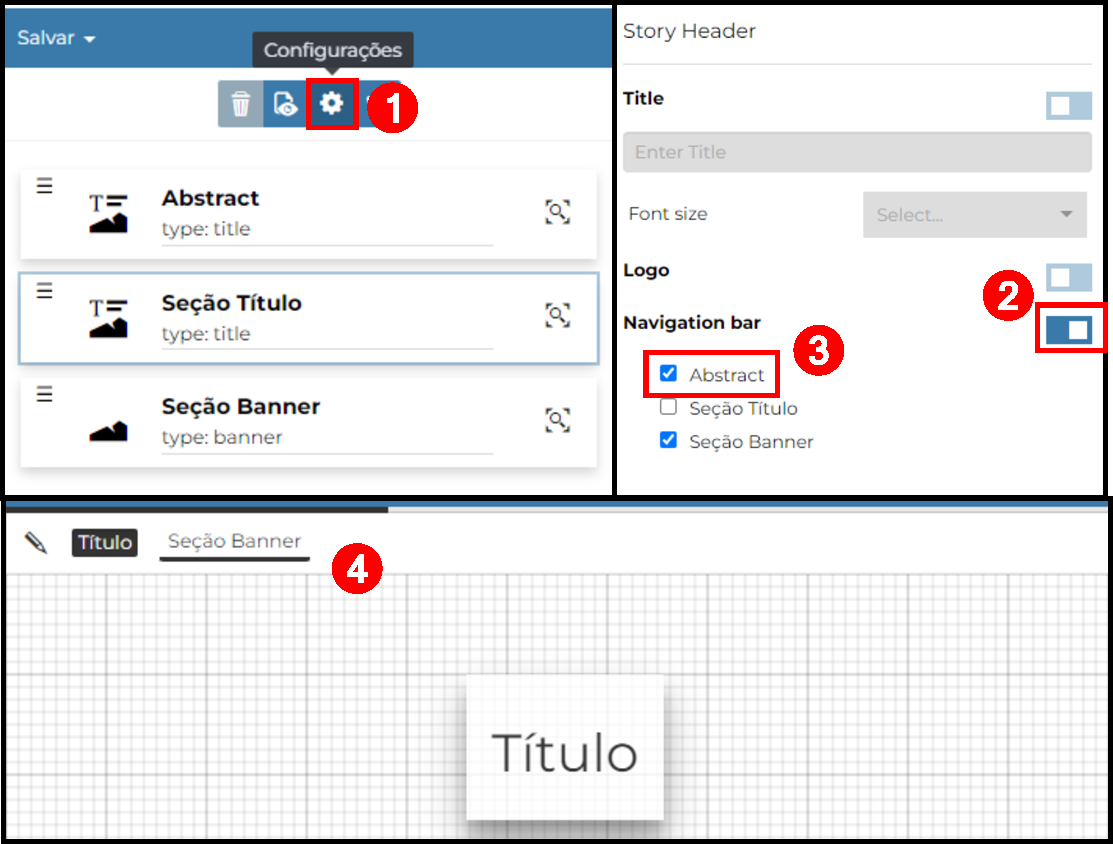
\includegraphics[width=\textwidth, keepaspectratio]{img/navegacaoGeostory.pdf}
    \caption{Configuração da barra de navegação de um Geostory.}
    \label{fig:navegacao}
  \end{figure}

\end{document}
